\documentclass{article}
\usepackage{graphicx, placeins, etoolbox, breakcites, cite, color, hyperref, dsfont, amssymb, rotating, booktabs, array , ragged2e, breqn, morefloats, chngcntr, tabularx, titling, lscape, multirow, subfig, longtable, pdflscape, adjustbox, threeparttable, wrapfig}
\usepackage[justification=centering]{caption}
\title{Stata-LaTeX Integration Example}
\author{J-PAL}
\date{Last Updated: November 2023}
\begin{document}
\maketitle
\begin{center}
\begin{threeparttable}
\caption{Descriptive Statistics}
\begin{tabular}{p{4.5cm}ccc}
\toprule \toprule
& Treatment & Control  \\
\midrule
 Pre-test Score & 32.32 & 32.88 \\ 
 Post-test Score & 43.58 & 40.88 \\ 
 Female & .51 & .52 \\ 
 Grade 3 & .52 & .49 \\ 
 Grade 4 & .48 & .51 \\ 
 Big School & .64 & .67 \\ 
\midrule
Observations & 4084  & 4342  \\ 
\bottomrule
\end{tabular}
\multicolumn{5}{l}{\footnotesize \emph{Notes:} Test scores can range from 0-100. }
\end{threeparttable}
\end{center}
\begin{center}
\begin{threeparttable}
\caption{Regression Results}
\begin{tabular}{p{3cm}ccccc}
\toprule \toprule
& & Post-test Score & \\
& Coefficient & P-value & Coefficient & P-value \\
\midrule
Balsakhi Treatment &  2.705  & 0.00 & 3.135 & 0.00 \\
& (.533)  &     &  (.51) &  \\
 Female  &   & &  2.292 & 0.00 \\ 
& & &  (.511)  &  \\
 Big School  &   & &  -2.042 & 0.00 \\ 
& & &  (.537)  &  \\
 Grade  &   & &  14.103 & 0.00 \\ 
& & &  (.51)  &  \\
\midrule
Observations & 8426  & &  8426 & \\ 
R^2 & .09  & &  .09 & \\ 
\bottomrule
\end{tabular}
\multicolumn{5}{l}{\footnotesize \emph{Notes:} Standard errors in parentheses. }
\end{threeparttable}
\end{center}
\begin{figure}[h]
\centering
\caption[online]{Improvement in test scores following program intervention, by pre-test score bin}
\begin{minipage}{1\textwidth}
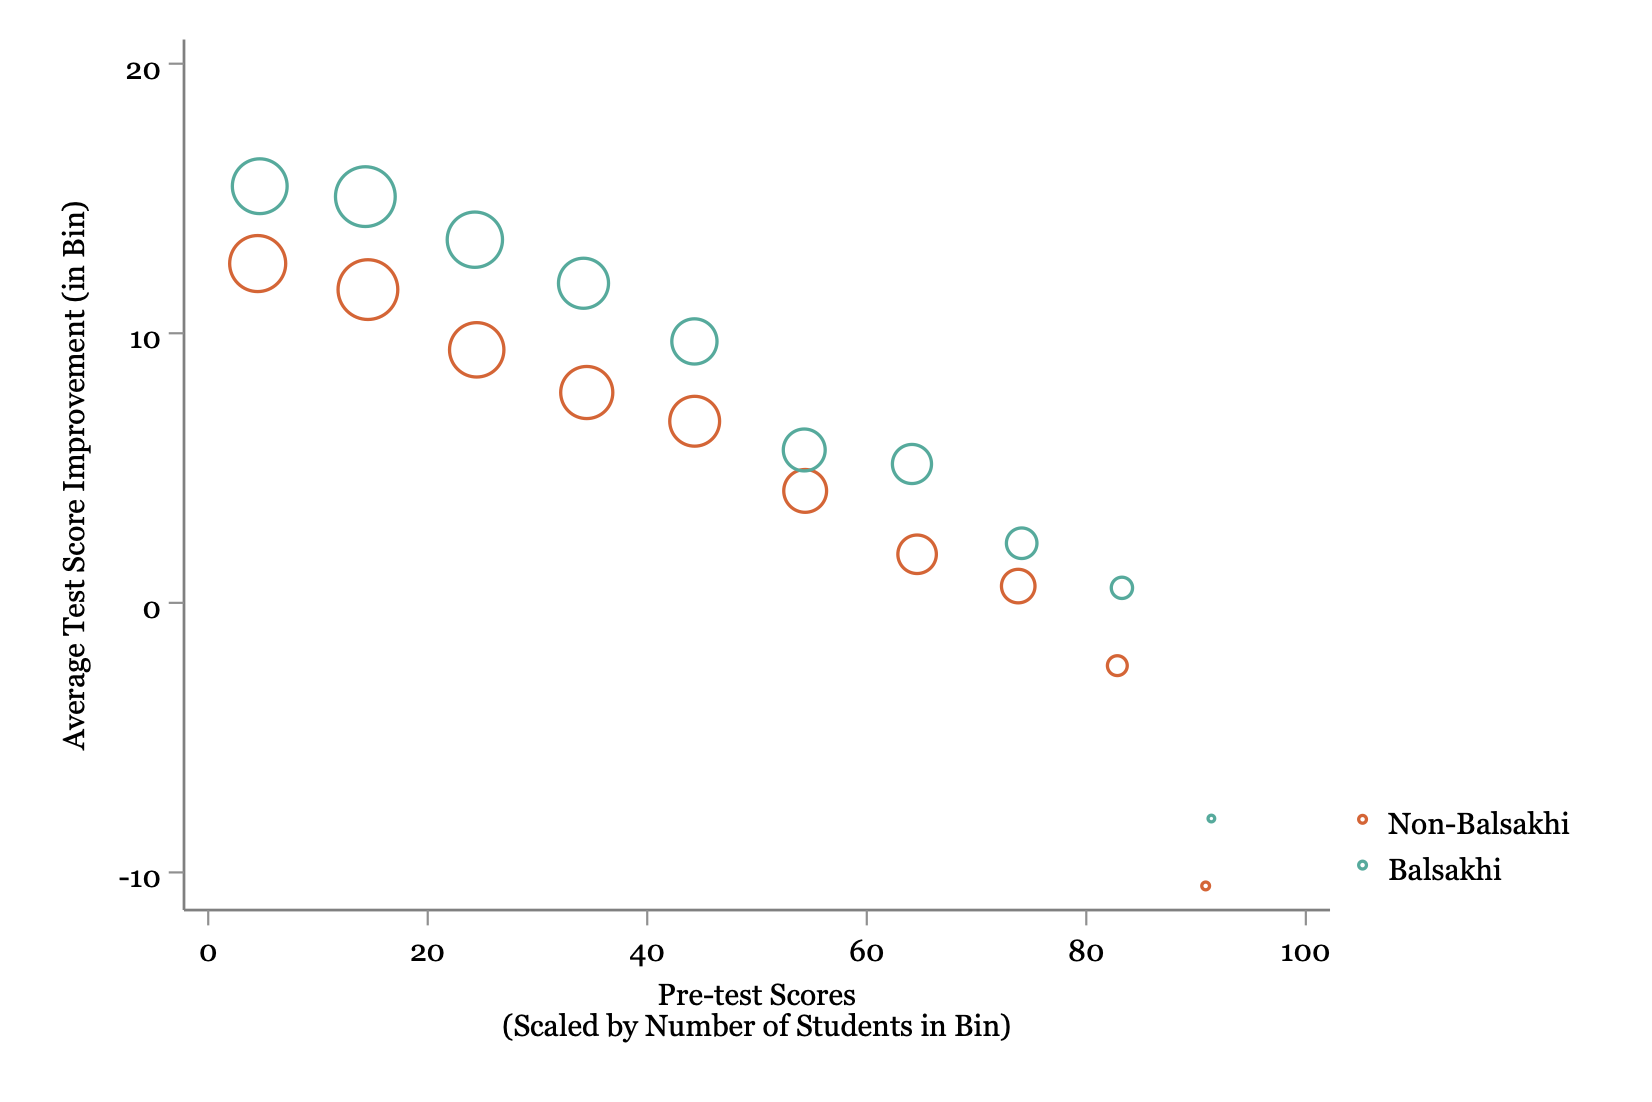
\includegraphics[width=1\linewidth]{./figures/figure_1.png}
{\footnotesize \emph{Notes:} Students are divided into 10 bins based on their pre-test scores. Markers are scaled by the number of students in each bin.\par}
\end{minipage}
\end{figure}
\end{document}
